\documentclass[a4paper,12pt]{article}
\usepackage[left=1.5cm,right=1.5cm,top=2cm,bottom=2.5cm]{geometry}
\usepackage[utf8]{inputenc}
\usepackage[T1]{fontenc}
\usepackage[french]{babel}

\usepackage{iftex}
\ifPDFTeX
  \usepackage{fourier}       % For pdfLaTeX (Type1 fonts)
\else
  \usepackage{fourier-otf}   % For LuaLaTeX or XeLaTeX (OpenType fonts)
\fi

% PDF
\usepackage{hyperref}
\hypersetup{colorlinks=true, linkcolor=blue, urlcolor=blue}

% Table
\usepackage{tabularx}
\usepackage{array}

% Image
\usepackage{graphicx}

% Texte fond coloré
\usepackage{xcolor}
% Couleurs des boutons Xbox
\definecolor{xbox_A_vert}{RGB}{0, 255, 0}
\definecolor{xbox_B_rouge}{RGB}{255, 0, 0}
\definecolor{xbox_X_bleu}{RGB}{0, 0, 255}
\definecolor{xbox_Y_jaune}{RGB}{255, 255, 0}
% Couleurs des symboles PlayStation (Sony)
\definecolor{ps_triangle_vert}{RGB}{0, 158, 96}
\definecolor{ps_rond_rouge}{RGB}{224, 45, 45}
\definecolor{ps_croix_bleu}{RGB}{60, 120, 216}
\definecolor{ps_carre_rose}{RGB}{214, 74, 141}

% Boutons PlayStation : le symbole Sony (couleur d'origine) dans un cercle a bord
% noir, comme un bouton rond de la manette. Dessines au trait (TikZ) plutot qu'avec
% \square (amssymb), qui entre en conflit avec fourier-otf (\eth deja defini). Le
% cercle a le meme diametre (2ex) que les disques Xbox ; baseline -0.6ex pour
% rester centre sur la ligne du tableau. Coordonnees en ex, centrees sur (0,0).
\usepackage{tikz}
\newcommand{\symtriangle}{\tikz[baseline=-0.6ex]{%
  \draw[black,line width=0.5pt] (0,0) circle (1ex);
  \draw[ps_triangle_vert,line width=0.7pt] (0,0.42ex) -- (-0.4ex,-0.32ex) -- (0.4ex,-0.32ex) -- cycle;}}
\newcommand{\symrond}{\tikz[baseline=-0.6ex]{%
  \draw[black,line width=0.5pt] (0,0) circle (1ex);
  \draw[ps_rond_rouge,line width=0.7pt] (0,0) circle (0.42ex);}}
\newcommand{\symcroix}{\tikz[baseline=-0.6ex]{%
  \draw[black,line width=0.5pt] (0,0) circle (1ex);
  \draw[ps_croix_bleu,line width=0.7pt] (-0.4ex,-0.4ex) -- (0.4ex,0.4ex) (-0.4ex,0.4ex) -- (0.4ex,-0.4ex);}}
\newcommand{\symcarre}{\tikz[baseline=-0.6ex]{%
  \draw[black,line width=0.5pt] (0,0) circle (1ex);
  \draw[ps_carre_rose,line width=0.7pt] (-0.36ex,-0.36ex) rectangle (0.36ex,0.36ex);}}

% Bouton Xbox : disque de couleur avec la lettre au centre (comme les boutons
% ronds de la manette). Dessine avec TikZ, hauteur bornee (minimum size en ex) et
% baseline reglee pour que la pastille reste centree sur la ligne sans deborder
% sur les filets du tableau. #1 = couleur du disque, #2 = couleur de la lettre,
% #3 = lettre.
\newcommand{\boutonxbox}[3]{%
  \tikz[baseline=-0.6ex]{\node[circle, fill=#1, text=#2,
      font=\ttfamily\scriptsize\bfseries, inner sep=0.25ex,
      minimum size=2ex] at (0,0) {#3};}%
}

% Bloc de titre repris a l'identique sur chaque version (Xbox puis PlayStation).
% \maketitle ne peut servir qu'une seule fois : on definit notre propre bloc pour
% pouvoir reprendre exactement le meme titre en tete de la partie PlayStation.
% Version affichee sous le titre : numero de la derniere release suivi du commit
% courant (ex. 0.8.0.16c610f). La chaine est generee par build.sh -d dans
% docs/version.tex ; en son absence (compilation manuelle), on retombe sur une
% valeur par defaut.
\InputIfFileExists{version.tex}{}{}
\providecommand{\noticeversion}{version de développement}

\newcommand{\titrenotice}{%
  \begin{center}
    {\LARGE\bfseries Simulateur Aérospatiale Alouette II SE.3130}\\[1.5ex]
    {\large Olivier Booklage}\\[0.5ex]
    version \noticeversion
  \end{center}%
}

\begin{document}

% ==================== Version manette Xbox (2 pages) ====================
\titrenotice

\begin{center}\large\textbf{Manette Xbox}\end{center}

\begin{center}
	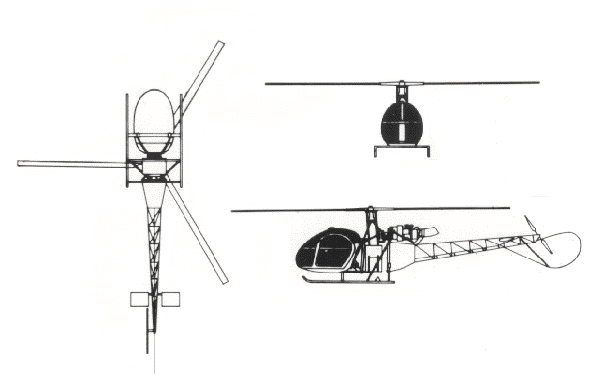
\includegraphics[scale=0.4]{Aérospatiale_Alouette_II_schema.png}
\end{center}

\section*{Introduction}
Ce document décrit les commandes disponibles pour piloter le simulateur Artouste, tant au clavier qu'avec une manette de jeu \textbf{Xbox} USB ou Bluetooth.

\section{Commandes de vol}

\begin{tabularx}{\linewidth}{|>{\raggedright\arraybackslash}X|>{\raggedright\arraybackslash}X|>{\raggedright\arraybackslash}X|}
\hline
\textbf{Action} & \textbf{Clavier AZERTY} & \textbf{Manette Xbox} \\
\hline
Turbine (d\'emarrer / couper) & T & bouton \texttt{Start} \\
\hline
Collectif +/- & Z (monter) / S (descendre) & RT / LT \\
\hline
Cyclique & Fl\`{e}ches directionnelles & stick gauche \\
\hline
Recentrer le cyclique & Espace & - \\
\hline
Palonnier & D / Q & stick droit\\
\hline
Mode assist\'e (confort) & M & LB \\
\hline
Pause & P & bouton \texttt{Back} \\
\hline
\end{tabularx}

\medskip
\noindent
\footnotesize\emph{Les touches indiquées correspondent à un clavier \textbf{AZERTY} français : Z, S, Q et D forment le losange de pilotage (collectif Z/S, palonnier Q/D). Sur un clavier \textbf{QWERTY}, ces mêmes emplacements physiques portent les lettres W, S, A et D ; le simulateur reconnaît les deux positions.}\normalsize

\newpage
\section{Autres commandes}

\begin{tabularx}{\linewidth}{|>{\raggedright\arraybackslash}X|>{\raggedright\arraybackslash}X|>{\raggedright\arraybackslash}X|}
\hline
\textbf{Action} & \textbf{Clavier AZERTY} & \textbf{Manette Xbox} \\
\hline
Vue (4 vues) & C & bouton \boutonxbox{xbox_Y_jaune}{black}{Y} \\
\hline
Livr\'ee & L & bouton \boutonxbox{xbox_A_vert}{black}{A} \\
\hline
Mode assist\'e (confort) & M & LB \\
\hline
Atterrissage automatique & J & RB \\
\hline
HUD (3 modes) & H & bouton \boutonxbox{xbox_B_rouge}{white}{B} \\
\hline
Plein \'ecran (fen\^etr\'e / plein \'ecran) & F & - \\
\hline
Pause & P & bouton \texttt{Back} \\
\hline
Radio internet (allumer / couper) & K & - \\
\hline
Balance radio / h\'elico & - / + & - \\
\hline
Reset position & R & bouton \boutonxbox{xbox_X_bleu}{white}{X} \\
\hline
D\'emo (lancer depuis le menu / en sortir) & D au menu ; \texttt{\'Echap} pour sortir & bouton \boutonxbox{xbox_Y_jaune}{black}{Y} au menu ; LB + RB pour sortir \\
\hline
Retour au menu (quitter depuis le menu) & \texttt{\'Echap} & LB + RB \\
\hline
\end{tabularx}

\clearpage

% ================= Version manette PlayStation (2 pages) =================
% Meme titre repris a l'identique. On remet le compteur de sections a zero pour
% que cette partie soit numerotee comme la precedente (1. Commandes de vol, etc.),
% et le compteur de page a 1 : la partie PlayStation forme une notice a part
% entiere, numerotee page 1 et page 2.
\setcounter{section}{0}
\setcounter{page}{1}
\titrenotice

\begin{center}\large\textbf{Manette PlayStation}\end{center}

\begin{center}
	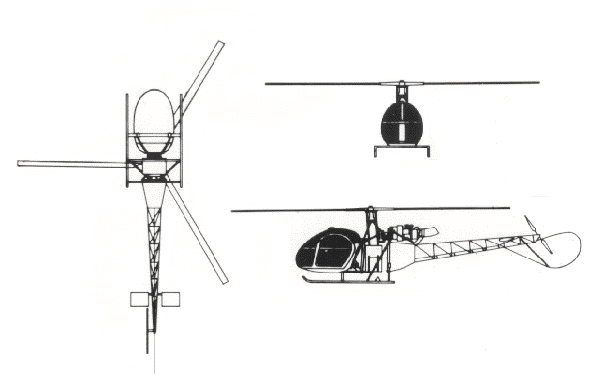
\includegraphics[scale=0.4]{Aérospatiale_Alouette_II_schema.png}
\end{center}

\section*{Introduction}
Ce document décrit les commandes disponibles pour piloter le simulateur Artouste, tant au clavier qu'avec les manettes de jeu \textbf{PlayStation 4 (DualShock 4)} ou \textbf{PlayStation 5 (DualSense)} USB ou Bluetooth.

\section{Commandes de vol}

\begin{tabularx}{\linewidth}{|>{\raggedright\arraybackslash}X|>{\raggedright\arraybackslash}X|>{\raggedright\arraybackslash}X|}
\hline
\textbf{Action} & \textbf{Clavier AZERTY} & \textbf{Manette PlayStation} \\
\hline
Turbine (d\'emarrer / couper) & T & bouton \texttt{Options} \\
\hline
Collectif +/- & Z (monter) / S (descendre) & R2 / L2 \\
\hline
Cyclique & Fl\`{e}ches directionnelles & stick gauche \\
\hline
Recentrer le cyclique & Espace & - \\
\hline
Palonnier & D / Q & stick droit\\
\hline
Mode assist\'e (confort) & M & L1 \\
\hline
Pause & P & bouton \texttt{Share} / \texttt{Create} \\
\hline
\end{tabularx}

\medskip
\noindent
\footnotesize\emph{Les touches indiquées correspondent à un clavier \textbf{AZERTY} français : Z, S, Q et D forment le losange de pilotage (collectif Z/S, palonnier Q/D). Sur un clavier \textbf{QWERTY}, ces mêmes emplacements physiques portent les lettres W, S, A et D ; le simulateur reconnaît les deux positions.}\normalsize

\newpage
\section{Autres commandes}

\begin{tabularx}{\linewidth}{|>{\raggedright\arraybackslash}X|>{\raggedright\arraybackslash}X|>{\raggedright\arraybackslash}X|}
\hline
\textbf{Action} & \textbf{Clavier AZERTY} & \textbf{Manette PlayStation} \\
\hline
Vue (4 vues) & C & bouton \symtriangle{} \\
\hline
Livr\'ee & L & bouton \symcroix{} \\
\hline
Mode assist\'e (confort) & M & L1 \\
\hline
Atterrissage automatique & J & R1 \\
\hline
HUD (3 modes) & H & bouton \symrond{} \\
\hline
Plein \'ecran (fen\^etr\'e / plein \'ecran) & F & - \\
\hline
Pause & P & bouton \texttt{Share} / \texttt{Create} \\
\hline
Radio internet (allumer / couper) & K & - \\
\hline
Balance radio / h\'elico & - / + & - \\
\hline
Reset position & R & bouton \symcarre{} \\
\hline
D\'emo (lancer depuis le menu / en sortir) & D au menu ; \texttt{\'Echap} pour sortir & bouton \symtriangle{} au menu ; L1 + R1 pour sortir \\
\hline
Retour au menu (quitter depuis le menu) & \texttt{\'Echap} & L1 + R1 \\
\hline
\end{tabularx}

\end{document}
